\chapter{Planificación e Seguimento}

A elaboración deste proxecto levouse a cabo durante catro periodos de tempo diferenciados e separados no tempo:

\begin{itemize}
  \item O verán do ano 2013 como parte do programa GSoC.
  \item O primeiro cuatrimestre do curso 2013/2014.
  \item O verán do ano 2014 novamento como parte do GSoC.
  \item O segundo cuatrimestre do curso 2014/2015.
\end{itemize}

Neste cápitulo trataremos a planificación do proxecto e como se levou a cabo neses catro períodos de tempo.

\section{Google Summer of Code 2013}
O tempo de programación do Google Summer of Code son aproximadamente 4 meses, un total de 15 semanas. Durante a edición de 2013 planificouse qeu se ía traballar 13 semanas. As dúas semanas restantes correponden a asistencia a GUADEC e ao comezo do ano lectivo universitario 2013/2014. Contase traballar aproximadamente 5 horas diarias polo que dá un total de 325 horas.

O programa GSoC pide os participantes reportes periodicos en forma de artigos en blogs así que estas serán as nosas iteracións a través das cales iremos recibindo feedback por parte dos futuros usuarios do aplicativo. En función deste feedback iremos modificando o programa. Neste caso empregouse un blog personal creado con anterioridade e de nome \href{http://aquelando.info}{Aquelando.info}. As publicacións deste blog así como as de moitos desenvolvedores do proxecto GNOME están ligadas con Planet GNOME, que é un agregador de blogs, polo que a súa difusión é moi alta. A perioricidade das publicacións e polo tanto das iteracións variará dunha a outra pero é de entre dúas e tres semanas.

Durante este GSoC fixeronse 5 iteracións que explicamos a continuación.

\subsection{Primeira Iteración: Análise, deseño xenérico e inicio da implementación}

A primeira iteración iniciouse o 13 de Xuño e rematouse o 30 de Xuño. O tratarse da primeira iteración dun programa fíxose unha analise das necesidades e un deseño xenerico da estrutura do programa.

\subsubsection{Análise e deseño}
Para o análise, instalamos e estudiamos algúns programas existentes e enviamos correos a listas de correo de equipos de tradución para obter ideas. Obtemos bastante resporta sobretodo por parte de xente do Proxecto Trasno. Unha vez que tiñamos claro que necesidades ten o noso programa fixemos un deseño xenerico da estrutura do programa. Este deseño saca a luz algúns conceptos que estarán presente durante toda a vida do programa como poden ser os \emph{consellos} e as \emph{pistas}.

\begin{figure}[h]
    \centering
    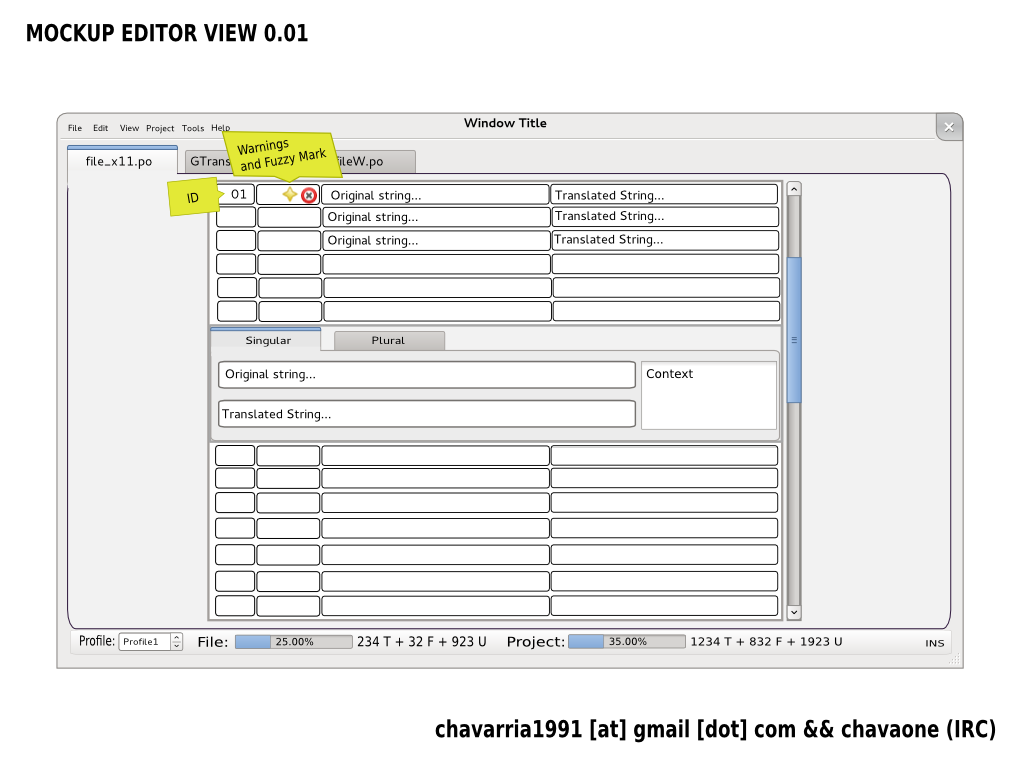
\includegraphics[width=\textwidth]{img/mockup_interface1.png}
    \caption{Mockup da interface presentado no reporte.}
    \label{fig:mockup_int1}
\end{figure}

Os consellos é un sistema lle amosa ao usuario posibles fallos que este tivo durante a tradución. Por outra pare as pistas son posibles traducións que se lle amosan ao usuario estas traducións poden vir de memorias de tradución, de outros linguaxes semellantes ou do propio ficheiro que se está a traducir, por exemplo.

Ademais tamén se fixo algun mockup da interface de usuario como o que se publicou no blog e se pode ver na Figura~\ref{fig:mockup_int1}. Estes deseños son bastante semellantes a interface do aplicativo Virtaal.

\subsubsection{Implementación da clase abstracta ficheiro}
Empeza a implementar parte do núcleo do sistema. Implementase unha clase abstracta ficheiro e unha clase \emph{DemoFile} que vai servir como mock para poder implementar a interface.

Esta clase implementase tendo en mente o concepto de extensibilidade xa que este programa aínda que se centra na edición de ficheiros PO por ser estes os "oficiais" de GNOME tamén queremos que este programa sexa útil para a comunidade de traductores en xeral.

\subsubsection{Reporte e feedback}
Escribironse un total de 3 reportes. Un\footnote{\href{http://aquelando.info/startinggsocprojec/}{Starting the GSoC Project!!}} facendo referencia as peticións obtidas por parte dos equipos de tradución e dous\footnote{\href{http://aquelando.info/valacat-some-design-aspects/}{ValaCAT. Some design aspects}}\footnote{\href{http://aquelando.info/valacat-some-design-aspects-part-2/}{ValaCAT. Some design aspects (Part 2)}} con algúns detalles que se tiveron en conta durante o deseño do programa. Houbo bastantes comentarios no blog e entre outras cousas os usuarios destacaron:

\begin{itemize}
  \item A importancia de non usar o patrón Singleton.
  \item Non facer os widgets dependentes da aplicación para que estos poidan ser reutilizados en outras aplicacións como Anjuta.
  \item Usar gettext-po para implementar os ficheiros po.
  \item Empregar unha interface máis semellante a anterior de GTranslator.
  \item Eliminar a columna de ID pois non se consider útil.
  \item Autoexpandir o tamaño dos campos cando as cadeas sexan grandes.
\end{itemize}

Con respecto a estas ideas modificouse a interface que se ía facer para buscar un deseño moi parecido ao de GTranslator empregando ingluso a mesma biblioteca GNOME Docking Library que permite modificar os bloques da interface. Ademais eliminouse por completo o ID da cadea da interface. En canto a biblioteca gettext-po xa tiñamos en mente empregala.

\subsubsection{Tarefas e seguimento}

As tarefas que se realizaron durante esta iteración foron as seguintes:

\begin{itemize}
  \item Análise de Requisitos
    \begin{itemize}
      \item Estudio de ferramentas existentes.
      \item Enviar correos a diferentes equipos de traductores.
      \item Analizar respostas dos equipos.
    \end{itemize}
  \item Deseño xenerico do aplicativo.
  \item Deseño e implementación do ficheiros xenérico.
  \item Escribir primeiros reportes.
\end{itemize}

Planificaronse un total de 50 horas e fixeronse 60 debido a ter que esperar por que os traductores deran as súas opinións.

\subsection{Segunda Iteración: Linguaxes, Filtros e Interface}

A segunda iteración durou dende o 1 de Xullo ata o 18 de Xullo. Nesta iteración profundizase no núcleo do sistema e empezamos a traballar na interface de ususario.

\subsubsection{Linguaxes}
Implementación da clase linguaxe e da clase forma plural. Fixemos un par de ficheiros con cada linguaxe e con cada forma plural existente. A idea detras destes ficheiros é engadir información adicional a cada linguaxe e a cada forma plural. 

Nas formas plurais incluimos unhas etiquetas para explicar en forma de texto a que corresponde cada tipo de plural. Por exemplo para os plurais do galego, a forma plural 0 tería unha etiqueta ``Singular (1 elemento)'' e a forma plural tería a forma ``Plural (0 ou máis de 1 elementos)''. Desta forma resultará máis sinxelo identificar cada forma plural e non ter que usar só o número.

\subsubsection{Filtros para as cadeas}
Os filtros para as cadeas corresponde a idea de que cada consello poda incluir a función de resaltar certas partes da mensaxe para reforzar a información que nos dá. Estos filtros funcionan como un patrón decorador que colocan uns tags html antes e despois da parte resaltada de forma que despois se poda parsear esta información e mostrala ao usuario cambiando os estilos.

\subsubsection{Interface de usuario}
Empezase a traballar na interface do usuario. Nesta iteración crease a estrutura xeral e os widget de listar mensaxes, de editar mensaxes e de mostar o contexto da mensaxe. O aspecto final da interface despois desta iteración pódese ver na Figura~\ref{fig:gsoc1_iter2_ui}.

\begin{figure}[h]
    \centering
    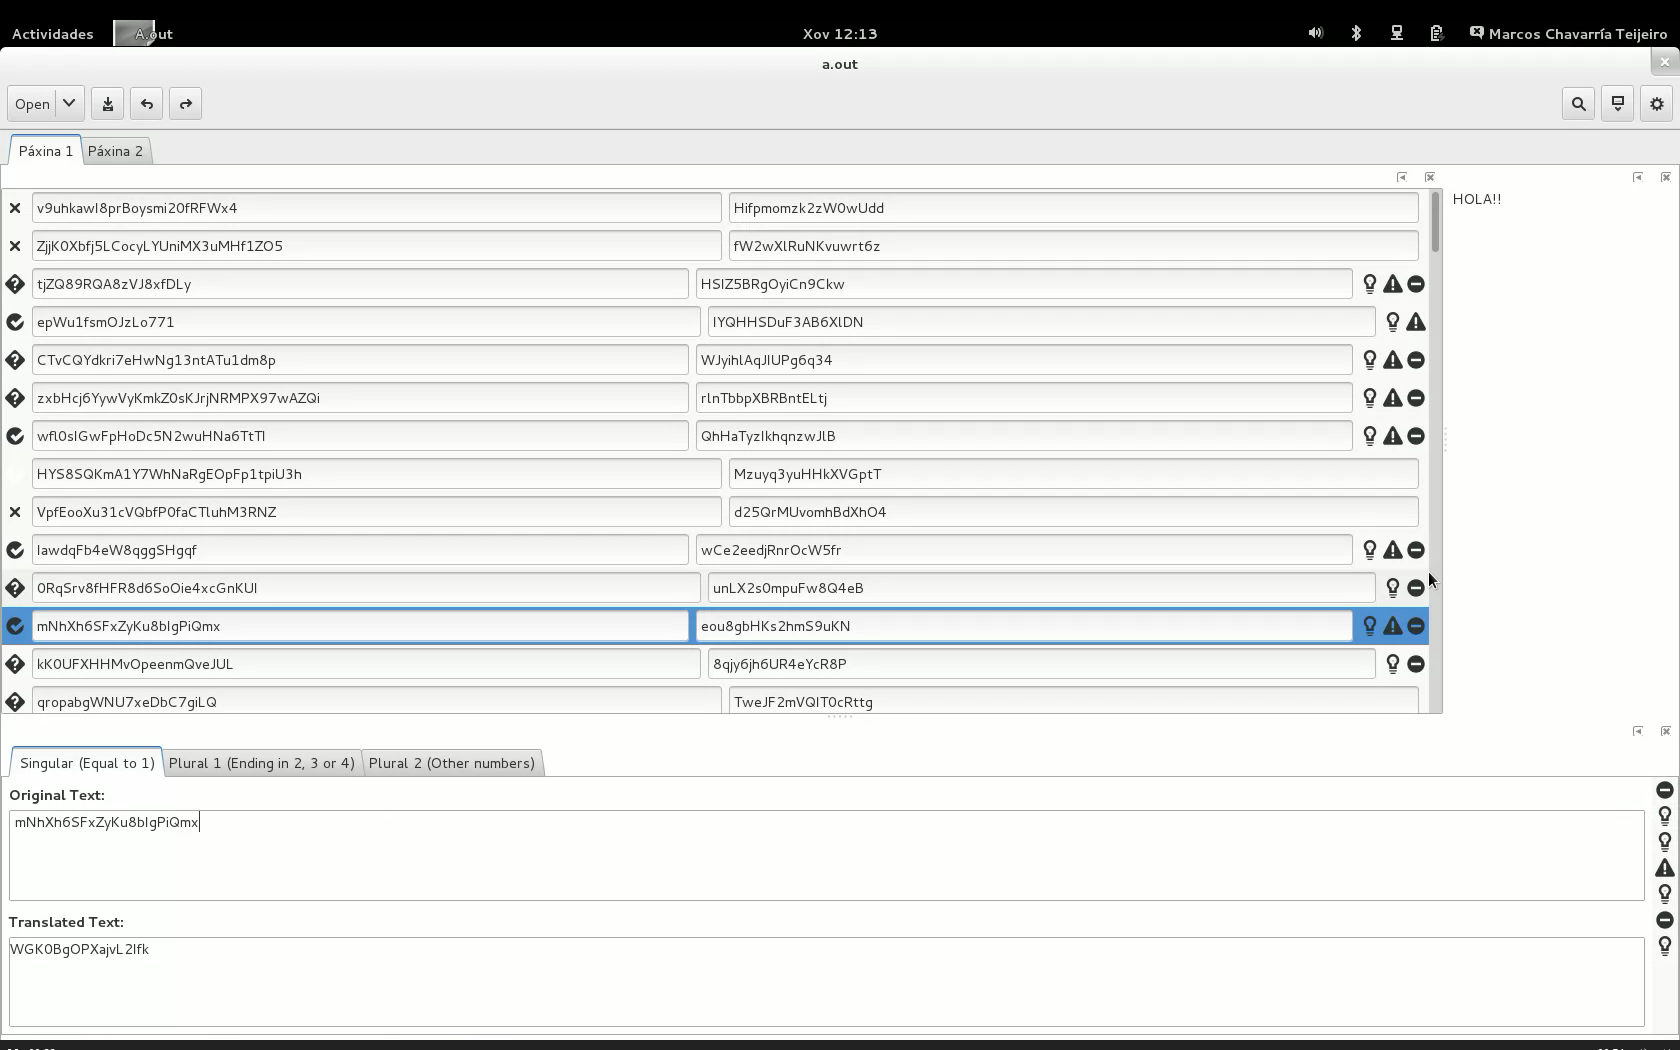
\includegraphics[width=0.8\textwidth]{img/gsoc1_it2_ui.png}
    \caption{Primeira implementación da interface.}
    \label{fig:gsoc1_iter2_ui}
\end{figure}

\subsubsection{Reporte e feedback}
Escribiuse un\footnote{\href{http://aquelando.info/valacat-application-current-status/}{ValaCAT application current status}} reporte onde se puxo un vídeo no que se amosaba o estado do programa e todas as caracteristicas implementadas. Recibimos un comentario preguntando para que sirven certas partes da aplicación que aparecen no vídeo e respondese explicando as ideas empregadas e reforzandoo con outro video centrado nesas partes.

\subsubsection{Tarefas e Seguimento}

As tarefas que realizamos durante esta iteración foron as seguintes:

\begin{itemize}
  \item Deseño e Implementación do módulo de Linguaxes.
    \begin{itemize}
      \item Creación dos ficheiros JSON coa lista de formas plurais e de linguaxes.
    \end{itemize}
  \item Interface de usuario.
    \begin{itemize}
      \item Implementación da lista de mensaxes.
      \item Implementación do editor de mensaxes.
      \item Implementación da barra de estado.
      \item Implementación da lapela xenerica.
      \item Implementación da lapela para ficheiros.
    \end{itemize}
  \item Creación do Makefile
  \item Creación de filtros para as cadeas.
  \item Escribir reportes.
\end{itemize}

Planificaronse un total de 70 horas para esta iteración e completaronse en 75 horas. Estas horas fixeronse traballando máis horas ao día polo que non supuxo un desvio. 

\subsection{Terceira Iteración: Interface, iteradores e buscas}

\subsubsection{Iteradores e Buscas}
Os iteradores son o sistema empregado para navegar a través das cadeas do documento. Construironse de forma qeu o usuario puidese navegar a través de todas as cadeas, das cadeas sin traducir ou das cadeas con tradución difusa. Ademais creouse o módulo para buscar texto no documento.

\subsubsection{Interface de usuario}
Seguimos traballando na interface de usuario. Cambiamos o widget de edición para empregar a biblioreca GtkSourceView que incorpora un widget que permite resaltado de sintaxe, de espacios en blanco entreo outros. Ademais empezamos a usar a clase GtkAplication e GtkAplicationWindow. Os filtros son substituidos por GtkTextTags que estan integrados dentro da librería GTK. Engadimos un dialogo para facer buscas onde se poden selecionar distintos parametros sobre qeu cadeas incluir nas búsquedas.

\begin{figure}[h]
    \centering
    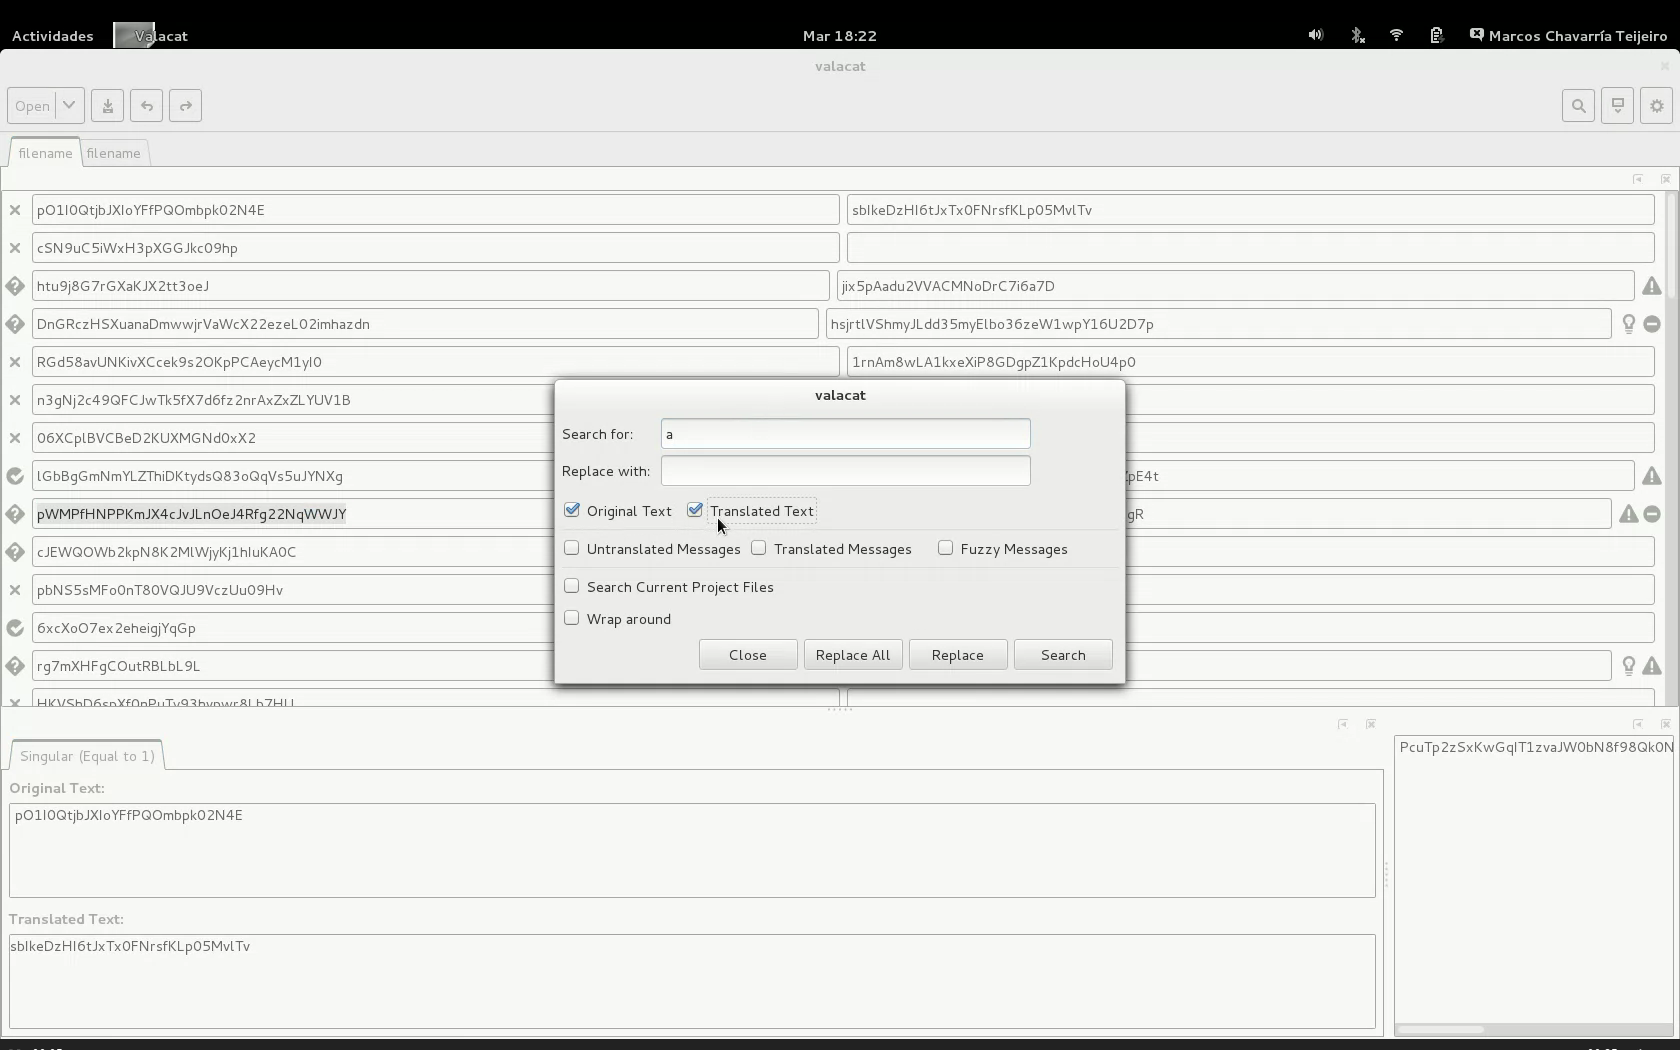
\includegraphics[width=0.8\textwidth]{img/gsoc1_it3_ui.png}
    \caption{Primeira implementación da interface.}
    \label{fig:gsoc1_iter3_ui}
\end{figure}

O aspecto que ten esta interface o finalizar esta iteración pódese ver na Figura~\ref{fig:gsoc1_iter3_ui}.

\subsubsection{Presentación GUADEC 2013 (Brno)}
A GUADEC e a xuntanza europea de desenvolvedores e usuarios de GNOME. Os participantes no GSoC están invitados a ir a dita reunión e expoñer o seu traballo nunha charla relámpago dun máximo de 3 minutos.

\begin{figure}[h!]
    \centering
    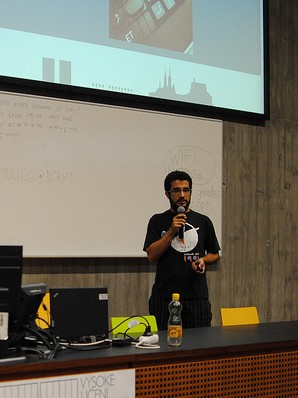
\includegraphics[width=0.275\textwidth]{img/guadec_2013_1.jpg}
    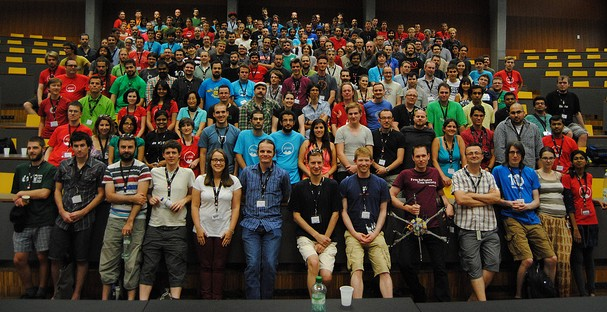
\includegraphics[width=0.715\textwidth]{img/guadec_2013_2.jpg}
    \caption{GUADEC 2013 (Brno)}
    \label{fig:guadec2012}
\end{figure}

Ademais de presentar o proxecto nesta xuntanza participei no evento como voluntario o que me permitiu coñecer a moita xente, algunha desa xente podo dicir que a día de hoxe son amigos meus.

\subsubsection{Reportes e Feedback}

A Fundación GNOME ponse en contacto conmigo a través do email para pedirme que, xa que esta vai ser o aplicativo oficial de GNOME, ten que ter a palabra GNOME no seu nome.

Escribironse dous reportes un\footnote{\href{http://aquelando.info/guadec-2013/}{GUADEC 2013}} falando da miña experiencia na GUADEC e outro\footnote{\href{http://aquelando.info/searching/}{Searching...}} falando dos avances no programa e pedindo ideas para o novo nome do aplicativo. Daniel Mustieles responde que ``GNOME Translator'' ou ``GNOME Translation Tool'' serían boas opcións.

\subsubsection{Tarefas e seguimento}

Nesta iteración continuamos traballando na interface, e implementaronse o sistema de navegación a través do documento e as buscas.

\begin{itemize}
  \item Deseño e implementación dos iteradores.
  \item Deseño e implementación do sistema de busca.
  \item Interface de usuario.
    \begin{itemize}
      \item Resaltado do texto ao facer click nos consellos.
      \item Modificar editor de mensaxes
    \end {itemize}
  \item Escribir reportes.
\end{itemize}

Esta iteración planificouse para un total de 50 horas e completouse en 60 horas debido ao tempo que tivemos que esperar polas respostas dos traductores e que se gastou analizando o código dos programas existentes.


\subsection{Cuarta Iteración: Ficheiros po, Autools, Proxectos, barra de busca}

\subsubsection{Ficheiros PO}
Ata este momento para probar a interface do programa viñamos empregando unha subclase da clase abstracta File de nome ``DemoFile'' e que funcionaba de \emph{mock} xerando aleatoriamente as cadeas. Agora implementamos o clase ``PoFile'' que representa un ficheiro po. Para facer esta implementación empregamos a biblioteca gettext-po.

Esta biblioteca está escrita en C polo que para usala con Vala temos que escribir uns bindings. Afortunadamente escribir uns bindings para Vala é bastante sinxelo se a biblioteca está escrita en C pois o propio Vala emprega C como linguaxe intermedio.

\subsubsection{Proxectos}
Un dos requisitos do programa é a aparición dos proxectos. Un proxecto é un conxunto de ficheiros que teñen algo en común e que estan na mesma carpeta. Nesta iteración implementamos este concepto.

\subsubsection{Autotools}
Durante a primeira iteración fixemos un pequeno script Makefile para compilar o programa mais según vai crecendo o aplicativo surxe a necesidade de usar un sistema de \emph{building} máis complexo. Escollese Autotools por varias recomendacións de outros desenvolvedores.

\subsubsection{Interface de usuario}
Continuamos traballando na interface. Engadese unha barra de busca e eleminase a barra de estado. Implementanse accións para facer e desfacer cambios, navegar a través do documento e outras cousas. Estas accións poderán ser activadasa a través de botóns na interface por agora e con atallos de teclado no futuro. Engádese soporte para abrir ficheiros dende a interface e ver os ficheiros recentes.

\subsubsection{Reportes e feedback}

Falando co anterior \emph{maintainer} de GTranslator a través de IRC, este aporta bastantes consellos sobre o programa como o uso de Autotools ou varios detalles da interface de usuario.

Realizaronse un total de dous reportes\footnote{\href{http://aquelando.info/gsoc-application-status-report/}{GSoC application status report}}\footnote{\href{http://aquelando.info/po-files-projects-navigation-and-other-stuff-i-have-been-doing/}{Po files, projects, navigation and other stuff I have been doing}} pero ninguén escribiu ningún comentario no blog.

\subsubsection{Tarefas e Seguimento}

As tarefas que se realizaron durante esta iteración foron as seguintes:

\begin {itemize}
  \item Implementación dos ficheiros po.
  \item Implementación de proxectos
  \item Implementación de accións
    \begin{itemize}
      \item Accións desfacer-refacer
      \item Accións de navegar polo documento.
    \end{itemize}
  \item Engadir barra de busca.
  \item Eliminar barra de estado.
  \item Substituir Makefile por Autools.
  \item Internacionalización do programa.
  \item Escribir reportes.
\end {itemize}

Planificaronse un total 90 horas para esta iteración e completouse en 110 horas debido as dificultades encontradas na implementación dos bindings da biblioteca de GetText e na implementación de Autotools. Estas horas alcanzaronse facendo máis horas cada día.

\subsection{Quinta Iteración: Preferencias, limpar código e documentación}
Durante esta iteración seguiuse traballando na interface, limpouse o código e creouse algo de documentación de cara a entraga final do Google Summer of Code.

\subsubsection{Preferencias}
Por agora moitas das opcións empregadas estaban \emph{hardcodeadas}, é dicir postas directamente no código. Para solucionar isto creamos as preferencias. Por un lado implementamos unha serie de preferencias empregando o compoñente de GLib GSettings que permite o almacenamento sinxelo de configuracíon das aplicacións mediante unha especie de tabla hash. Este compoñente permite o uso de diferentes \emph{backends} entre os cales destaca \emph{dconf} por ser o estandar de GNOME creado a tal efecto.

Ademais engadimos unha dialogo que permite editar estas preferencias dende o propio programa. Este dialogo copia os campos empregados anteriormete en GTranslator.

\begin{figure}[h]
    \centering
    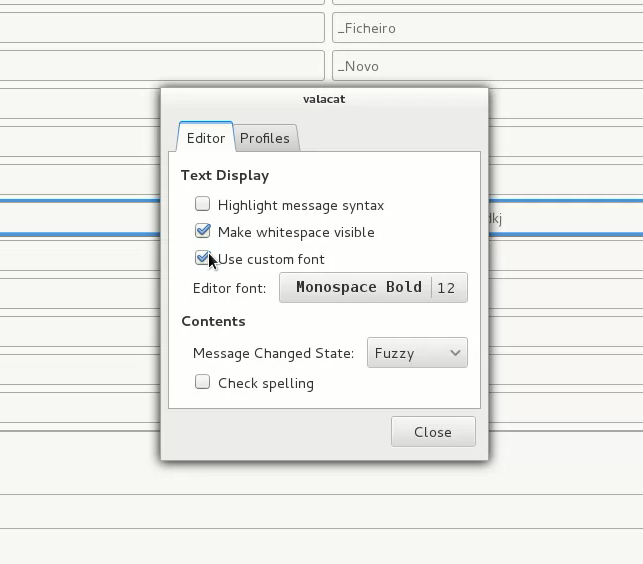
\includegraphics[width=0.7\textwidth]{img/gsoc1_it5_prefs.png}
    \caption{Diálogo de preferencias.}
    \label{fig:gsoc1_it5_prefs}
\end{figure}

Na Figura~\ref{fig:gsoc1_it5_prefs} pódese ver o aspecto deste dialogo.

\subsubsection{Mellorar a calidade do código e documentación}
Fixose unha revisión completa do código para manter un mesmo estilo ao largo de todo o código. Ademais actualizaronse os diagramas UML creados na primeira iteración.

\subsubsection{Reportes e Feedback}
Escibiuse un\footnote{\href{http://aquelando.info/gsoc-final-report/}{GSoC Final Report}} reporte onde se conta o estado da aplicación demostrandoo con un vídeo. O tratarse do último post desa edición do GSoC agradezo a oportunidade que me deu Google para poder estar ese verán traballando en software libre e describo a miña experiencia.

\subsubsection{Tarefas e seguimento}

As tarefas realizadas durante esta iteración foron as seguintes:

\begin {itemize}
  \item Deseño e implementación das preferencias.
  \item Correxir Clase ficheiro.
  \item Correxir errores de estilos no código.
  \item Actualizar diagramas UML.
  \item Escribir reportes.
\end {itemize}

Planificaronse un total de  horas para a realización destas tarefas.

\subsection{Estado ao fin do GSoC 2013}
O finalizar esta iteración o mentor do GSoC avalía correctamente o proxecto presentado polo que o programa é completado con éxito. O programa entregado ten entre outras moitas as seguintes características:

\begin{itemize}
  \item Posibilidade de abrir ficheiros po.
  \item Navegación a través do documento.
  \item Posibilidade de buscar.
  \item Editor con resaltado de sintaxe e de espacios en branco.
  \item Preferencias.
\end{itemize}

Pero tamén presenta algúns fallos:

\begin{itemize}
  \item Lentitude ao cargar ficheiros moi grandes.
  \item Fallo ao gardar un ficheiro.
  \item O aspecto da interface non é satisfactorio.
  \item Problemas ao buscar.
\end{itemize}

Intentamos durante o curso seguinte nos tempos libres arreglar estos fallos.

\section{Primeiro cuatrimestre curso 2013/2014}

Durante este periodo intetouse continuar o proxecto durante o tempo libre polo que estas iteracións son maís longas no tempo xa que tráballase un menor número de horas. Distinguimos dúas iteracións que corresponden a dous momentos durante o curso na que a carga de traballo permitiume seguir co proxecto.

\subsection{Primeira iteración: cambios na interface}
A primeira iteración comprende os últimos días de septembro e o mes de octubro. Durante este tempo faise un rediseño da interface gráfica e implementanse as pistas e os comprobadores.

\subsubsection{Interface Gráfica}
Decidimos facer un re-deseño da interface para intentar conseguir un mellor resultado. Para facer esto empregamos os deseños iniciais que se asemellan máis o aspecto da aplicación Virtaal.

Xa tiñamos feitos os widgets de edición e a lista de mensaxes polo que facer o novo deseño consiste en misturar os dous conceptos. Na Figura~\ref{fig:curso2014_it1_ui} podese ver o resultado. Desta forma se facemos click nun dos mensaxes da lista este expandese e permitenos editar o contido.

\begin{figure}[h!]
    \centering
    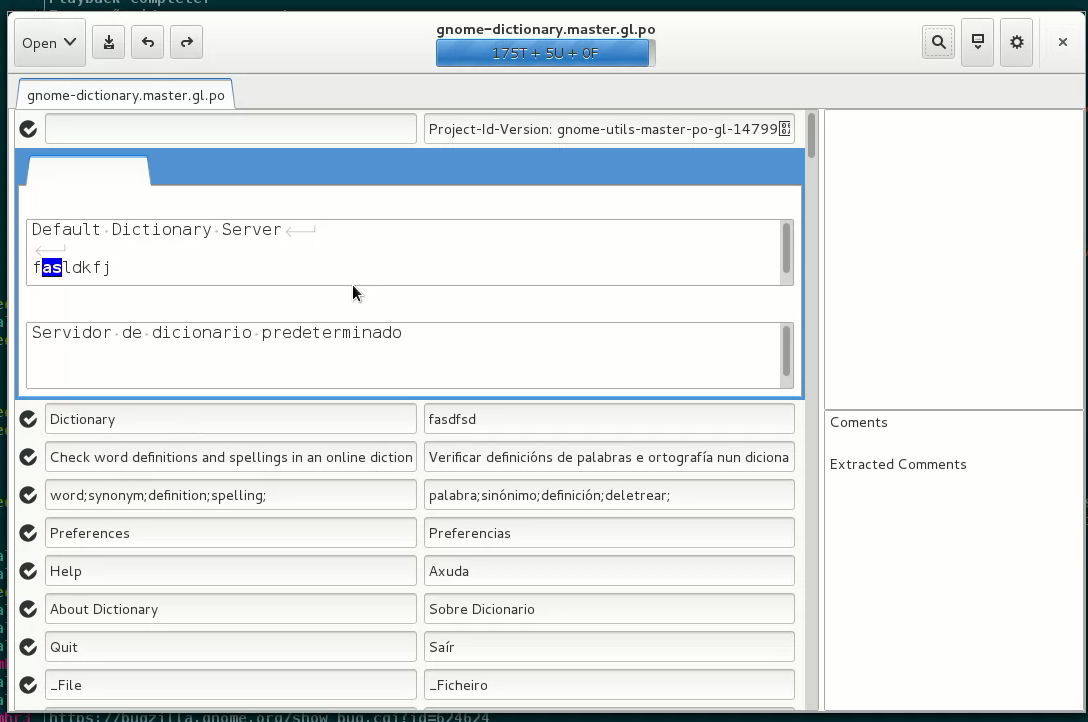
\includegraphics[width=0.8\textwidth]{img/curso2014_it1_ui.png} 
    \caption{Rediseño da interface}
    \label{fig:curso2014_it1_ui}
\end{figure}

Ademais deixamos de usar a biblioteca GDL xa que en conversacións a través de IRC chegouse a conclusión de que se o usuario tiña que usar esta biblioteca para modificar a interface isto é por que a interface está mal deseñada.


\subsubsection{Pistas e Comprobadores}
Como xa comentamos as pistas (\emph{hints}) son posibles traducións para unha cadea determinada. Nesta iteración creamos tanto o panel da interface que permite ver estas pistas como a clase que lle provee as pistas a dita interface. Por último creamos un mock para poder seguir traballando.

En canto aos comprobadores (\emph{checkers}), estos son os elementos do programa que aportan os consellos da mesma forma que cas pistas, implementamos a clase comprobador e crearmos un mock de nome \emph{DemoChecker}.

\subsubsection{Presentación GUADEC Hispana 2013 (Madrid)}

A GUADEC Hispana é unha reunión de usuarios e desarrolladores que falan castelán e que sirve tamén para a reunión anual (como obliga a lei) da organización GNOME Hispano. Ademais desta reunión fanse charlas sobre GNOME e outros temas relacionados.

\begin{figure}[h!]
    \centering
    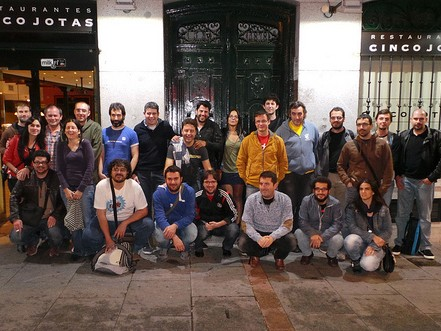
\includegraphics[width=0.495\textwidth]{img/guadec_es_2013_1.jpg}
    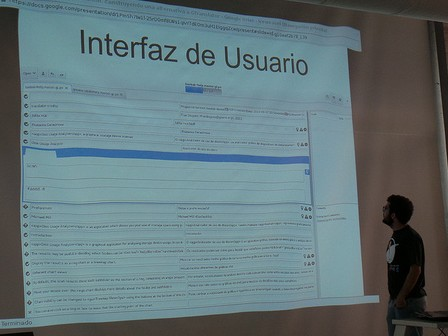
\includegraphics[width=0.495\textwidth]{img/guadec_es_2013_2.jpg} 
    \caption{GUADEC Hispana 2013 (Madrid)}
    \label{fig:guadec2012}
\end{figure}

Entre esas charlas deuse unha sobre o programa que se realiza neste proxecto na cal os asistentes amosaron o seu interese por que se seguira desenrolando.

\subsubsection{Reportes e feedback}
Escribiuse un reporte\footnote{\href{http://aquelando.info/changing-the-tool-ui/}{Changing the tool UI}} mais ninguén escribiu ningún comentario. Non obstante durante a GUADEC-es houbo xente que se interesou polo programa.

\subsubsection{Tarefas e seguimento}

As tarefas realizadas durante esta iteración foron as seguintes:

\begin{itemize}
  \item Implementar Pistas e Proveedor de Pistas.
  \item Implementar Comprobador.
  \item Interface de Usuario.
    \begin{itemize}
      \item Eliminar biblioteca GDL.
      \item Engadir widget de Pistas.
      \item Mezclar lista de mensaxes con editor de mensaxes.
    \end{itemize}
\end{itemize}

Para estas tarefas planificaronse 50 horas que se completaron con éxito.

\subsection{Segunda iteración: Refactorizar navegadores e melloras na interface}
Esta iteración sucede durante o mes de novembro e os primeiros días de decembro. Durante este tempo cambiase o nome do aplicativo, refactorizase a API para navegar a través do documento e realizanse pequenos cambios na interface de usuario.

\subsubsection{Refactorización dos navegadores}
Crease unha API a nivel de aplicación para movernos a través do documento. Implementa operacións para selecionar e tamén deselecionar cadeas e fragmentos destas cadeas a través de todo o documento.

\subsubsection{Cambio de nome}
Como nos pediron dende a GNOME Foundation, cambiamos o aplicativo de nome. O nome escollido o final é GNOMECAT. Eleximos este nome pois pensamos que o programa non é un traductor xa que non traduce el solo e isto pode levar a enganos. Para facer este cambio modificamos tanto o código como os ficheiros de configuración.

\subsubsection{Interface de usuario}
Aparte de solucionar alguns fallos do aplicativo fíxose un rediseño da opción buscar avanzado polo que se elminiou o dialogo e se engadiron estas opcións a barra de búsqueda. Na Figura~\ref{fig:curso2014_it2_search} pódese ver o resultado.

\begin{figure}[h!]
    \centering
    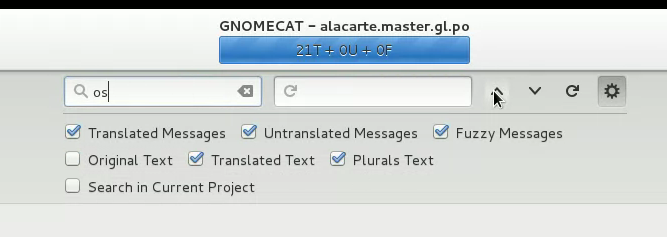
\includegraphics[width=0.7\textwidth]{img/curso2014_it2_search.png} 
    \caption{Buscar avanzado}
    \label{fig:curso2014_it2_search}
\end{figure}

\subsubsection{Reportes e Feedback}
Escribese un\footnote{\href{http://aquelando.info/welcome-gnomecat/}{Welcome GnomeCAT}} contando os últimos avances do aplicativo e o cambio de nome. Recibimos un comentario dicindo que GNOME escribese con letras maiusculas polo que temos que correxir o programa. Outra xente interesase polo significado de CAT.

\subsubsection{Tarefas e seguimento}

As tarefas realizadasa durante esta iteración foron as seguintes:

\begin{itemize}
  \item Cambiar nome do aplicativo.
  \item Refactorizar navegadores.
  \item Interface de usuario.
    \begin{itemize}
      \item Rediseño da opción buscar avanzado.
    \end{itemize}
\end{itemize}

\subsection{Presentación para o GSoC 2014}
Debido a evidente falta de tempo para completar o programa durante os ratos libres decidese presentar o programa de novo o proxecto Google Summer of Code. Falase coa cordinadora dos programas de iniciación en GNOME para saber se isto é posible e repondenos afirmativamente. Como mentor falamos co \emph{maintainer} de GTranslator que nos di que non ten ningún problema en facer de mentor. Presentamos o proxecto e este sale aceptado.

\section{Google Summer of Code 2014}
O Google Summer of Code durante o 2014 dura dende o 19 de maio ata o 11 de agosto un total de 15 semanas. Na planificación realizada contanse 13 semanas pois nunha das semanas o curso lectivo 2013/2014 aínda non acabou e na outra realizase o viaxe a GUADEC en Strasbourg. Da mesma forma que no caso anterior planeanse traballar 5 horas diarias o que da un total de 325 horas.

A maior experiencia no programa que estamos a facer permitenos facer unha planificación máis exacta. Faranse un total de cinco iteración de unha duración aproximada de duas semanas. 

%GSoC 2014 -> 19 de Maio - 11 Agosto -> 15 - 1 (guadec) - 1 (traballo r) -> 325h


\subsection{Primeira iteración: Rediseño UI}

Esta iteración dura dende o 23 de maio ata o 15 xuño. Durante ela fundamentalmente traballaremos nun rediseño da interface.

\subsubsection{Interface Gráfica}
O deseño anterior da interface non é plenamente satisfactorio polo que facemos unha vez máis un deseño da interface. Nesta ocasión intentamos contactar cos deseñadores de GNOME a través do chat IRC. 

Non obtemos demasiada axuda por parte dos deseñadores polo que decidimos empregar uns deseños feitos anteriormente para GTranslator e que nunca chegaron a estar implementados debido a falta de \emph{maintainer}. Baseandonos nas ideas expostas por estos deseños creamos un deseños para a maioría de dialogos da aplicación.

\begin{figure}[h!]
    \centering
    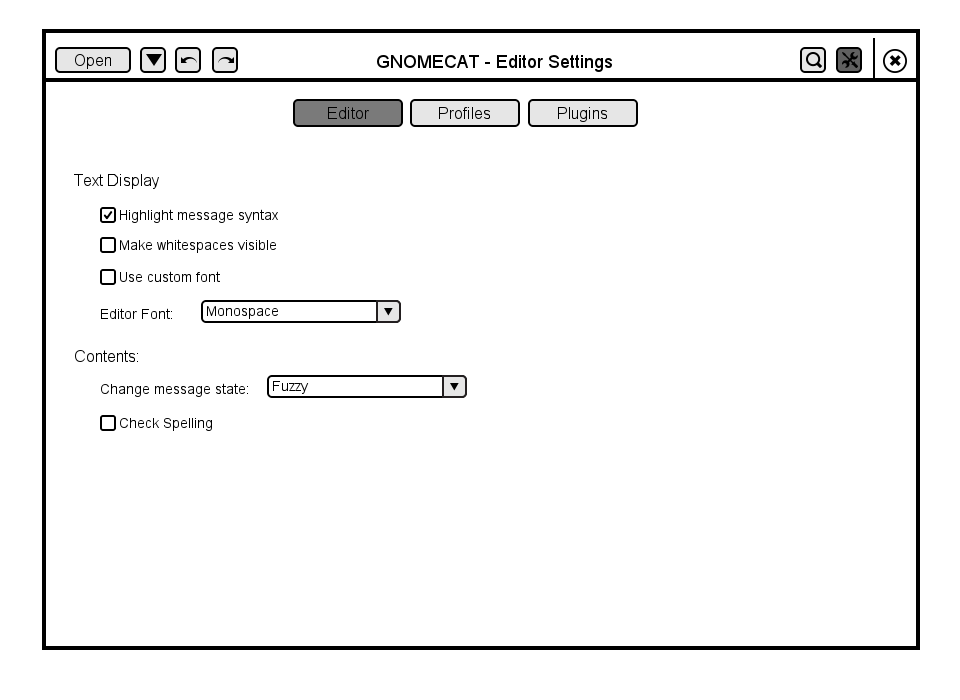
\includegraphics[width=0.9\textwidth]{img/gsoc2_it1_mockup.png} 
    \caption{Mockup para redeseño da interface de GNOMECAT}
    \label{fig:gsoc2_it1_mockup}
\end{figure}

En consonancia con outras interfaces de GNOME intentamos minimizar o uso de dialogos en forma de popups e facer que estas opción aparezan na ventá principal do aplicativo. Para iso creamos un sistema de paneis que se alternan dependendo da parte da aplicación estemos a usar. Creamos un panel de preferencias, un panel para editar os ficheiros, un para a lista de ficheiros abertos, un panel para abrir ficheiros, etc. Na Figura~\ref{fig:gsoc2_it1_mockup} podemos ver algún dos deseños empregados e na Figura~\ref{fig:gsoc2_it1_ui1} o resultado.

\begin{figure}[h!]
    \centering
    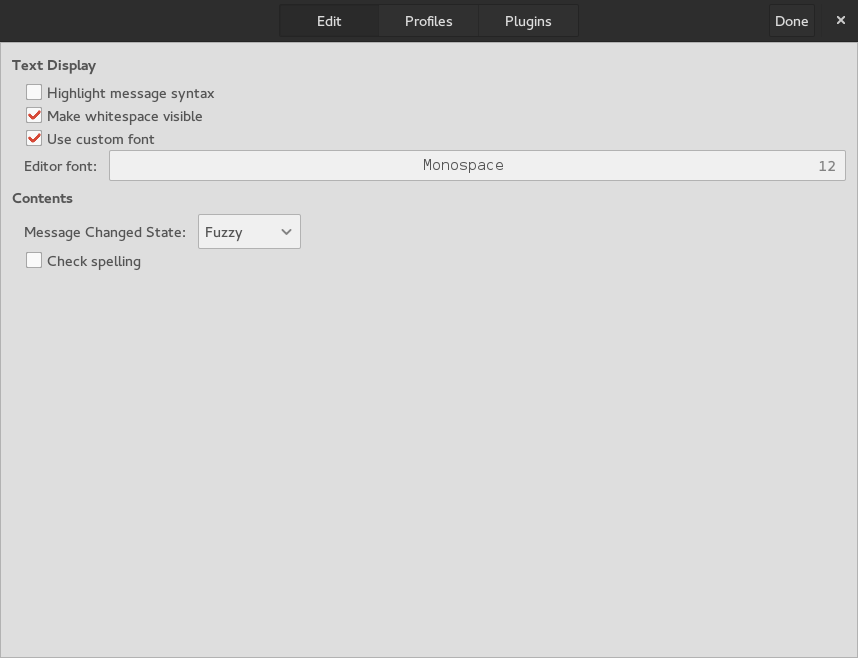
\includegraphics[width=0.9\textwidth]{img/gsoc2_it1_ui1.png} 
    \caption{Captura da vista de preferencias de GNOMECAT}
    \label{fig:gsoc2_it1_ui1}
\end{figure}

No panel de edición separamos o widget de lista de mensaxes e o widget que edita estos mensaxes. Prestamos especial antención a este último. A idea da interface e que darlle ao usuario moita información sobre a mensaxe que está a traducir e para facer isto, o widget de edición ocupa a maior parte da ventá. Os consellos irán aparecendo na parte superior da ventá segundo vamos editando para mostrarlle avisar ao usuario. Por último as pistas poderanse ver na zona dereita da pantalla. A nova interface pódese ver na Figura~\ref{fig:gsoc2_it1}.

\begin{figure}[h!]
    \centering
    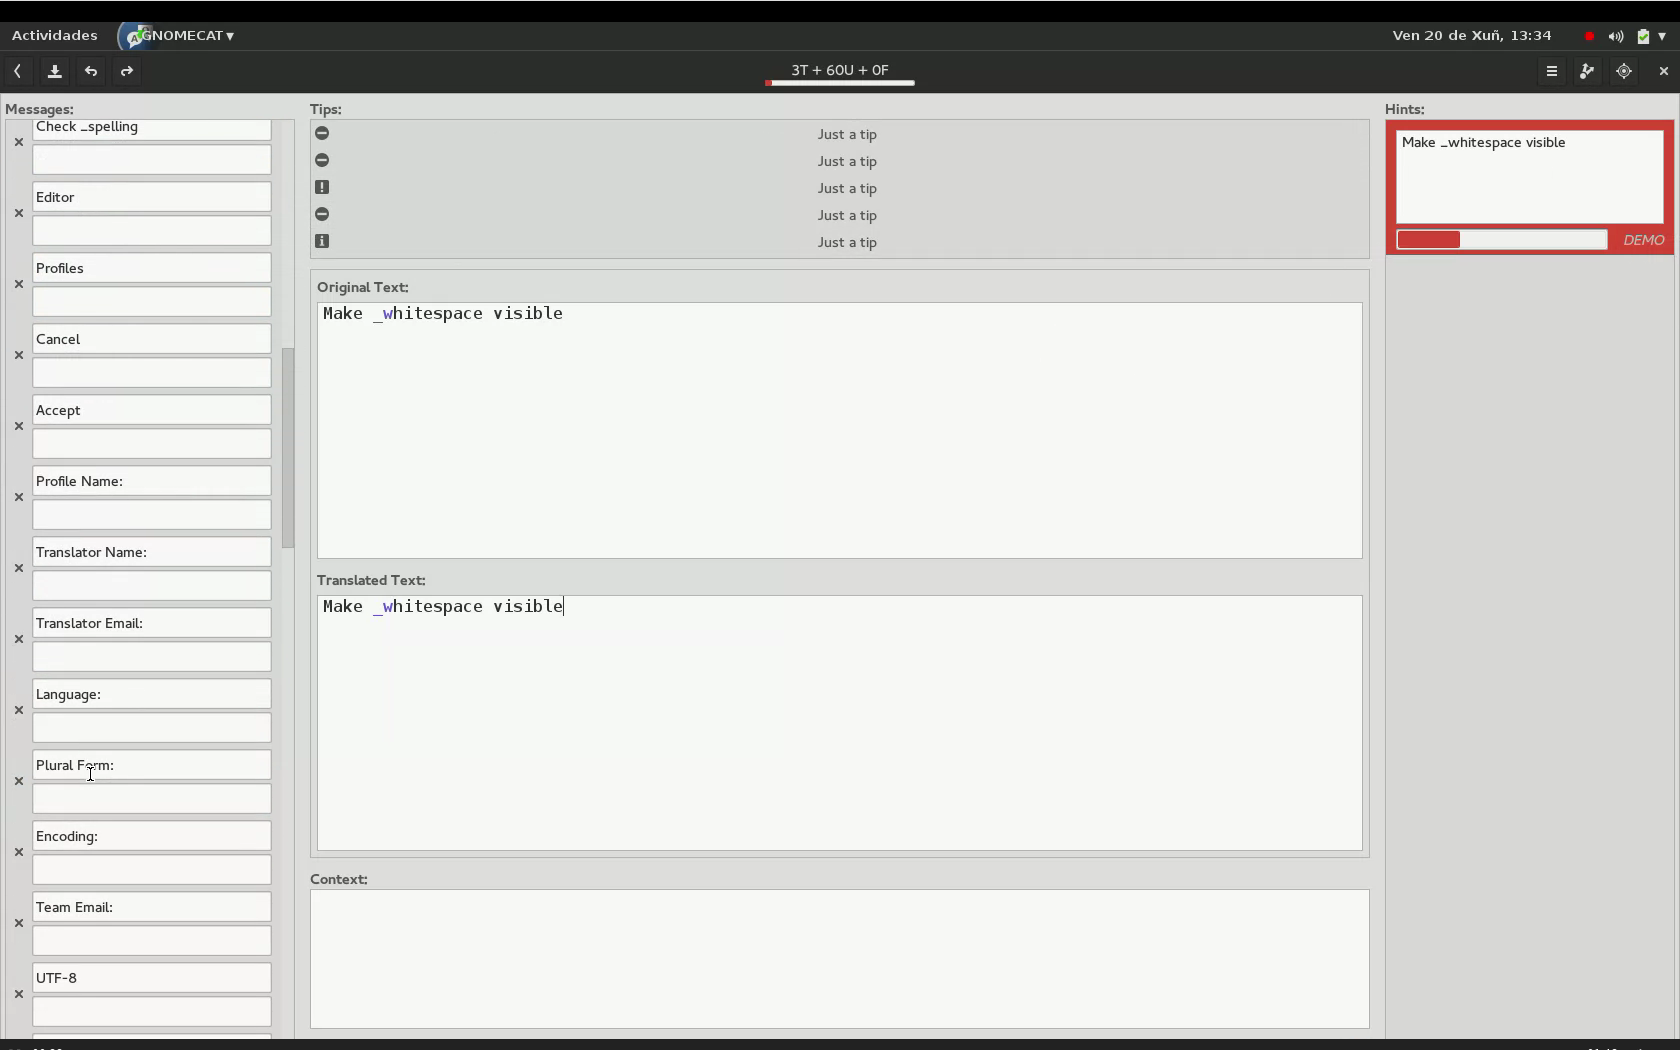
\includegraphics[width=0.9\textwidth]{img/gsoc2_it1_ui2.png} 
    \caption{Captura do panel de edición en GNOMECAT}
    \label{fig:gsoc2_it1_ui2}
\end{figure}

\subsubsection{Bindings Gettext-PO: Orixes das mensaxes}
A biblioteca gettext-po ten soporte para conseguir os orixes das mensaxes polo que melloramos os bindings para recoller esta característica e tamén a implementamos na clase PoFile engadindo a propiedade origins que permite obter en que ficheiros e liñas aparece dita cadea.

\subsubsection{Reportes e Feedback}
Escribironse dous\footnote{\href{http://aquelando.info/gnomecat-progress-report/}{GNOMECAT. Progress report}}\footnote{\href{http://aquelando.info/implementing-the-editing-panel/}{Implementing the Editing Panel}} reportes.

\subsubsection{Tarefas e seguimento}

As tarefas realizadas durante esta iteración foron:

\begin{itemize}
  \item Creación do ficheiro .desktop.
  \item Mellora de Autotools: xeneración automatica das cadeas a traducir.
  \item Interface de Usuario.
    \begin{itemize}
      \item Nova estrutura xeral.
      \item Creación da barra de ferramentas.
      \item Panel de edición.
      \item Panel de preferencias.
      \item Panel de perfil.
      \item Panel de benvida.
      \item Menu de aplicativo.
    \end{itemize}
  \item Bindings Gettext-PO: implementación das orixes dos mensaxes.
  \item Refactorización das buscas.
  \item Refactorización as formas plurais.
\end{itemize}

\subsection{Segunda Iteración: Bindings Gettext-PO e interface}
Esta iteración dura dende o 21 de xuño ata o 6 de xuño. Continuamos mellorando a interface de usuario, implementamos atallos de teclado e engadimos funcionalidade aos bindings de Gettext-PO.

\subsubsection{Interface de usuario}
Implementaronse atallos de teclado para poder navegar a través do documento e para outras funcións como salvar o ficheiro e buscar. Ademis implementamos a suxerencia feita no último reporte que indicaba facer intercambiables os botóns de gardar e de volver a lista de ficheiros.

\begin{figure}[h!]
    \centering
    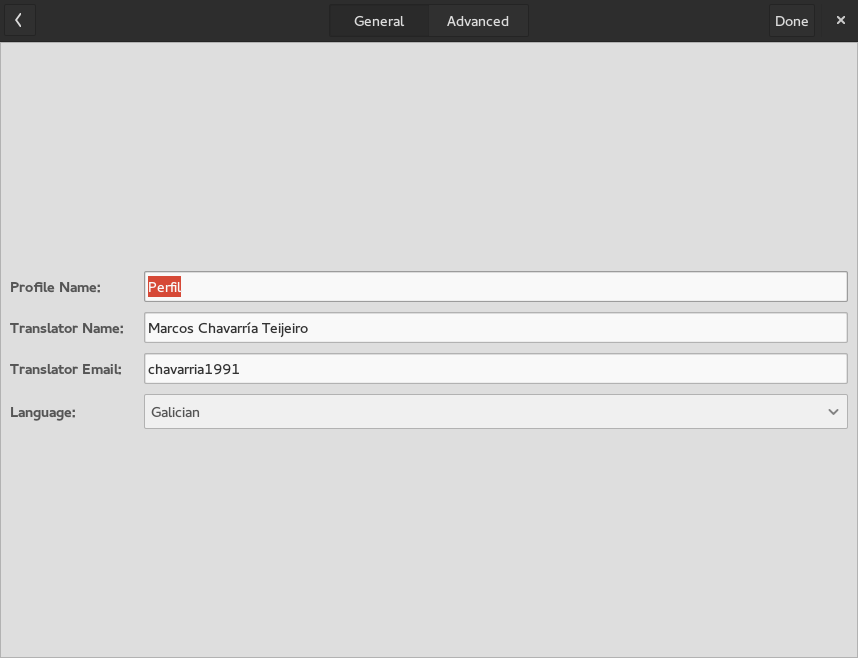
\includegraphics[width=0.49\textwidth]{img/gsoc2_it2_ui1.png}
    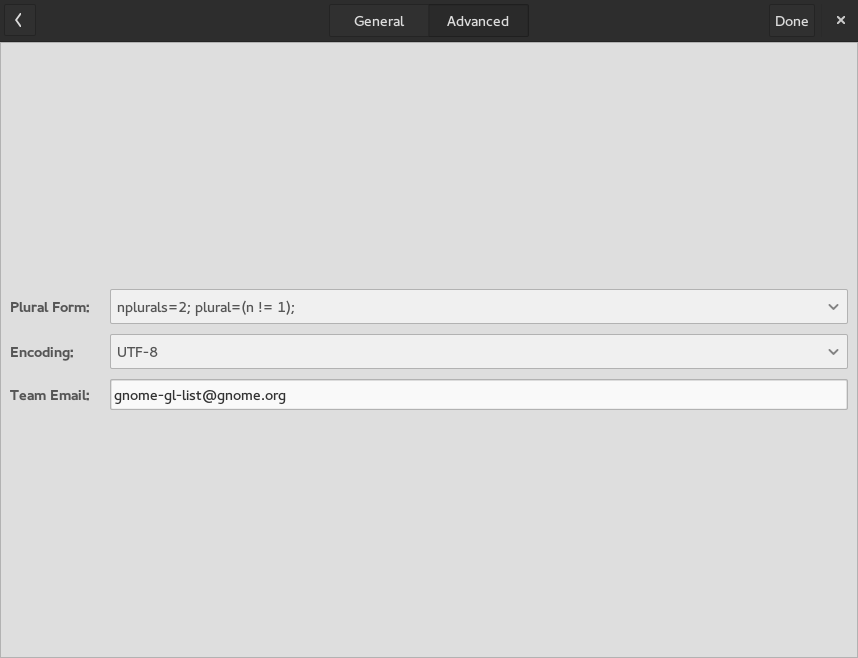
\includegraphics[width=0.49\textwidth]{img/gsoc2_it2_ui2.png}
    \caption{Novo panel de creación e edición de usuarios.}
    \label{fig:gsoc2_it2_ui1}
\end{figure}

Por outra parte melloramos notablemente o panel de crear ou editar perfiles de usuarios dividindo en dous subpaneles e facendo que ao selecionar un idioma as opcións de email do equipo de tradución e a forma de plural autocompletanse. Desta forma é máis sinxelo e máis rápido completar estos formularios. Na Figura~\ref{fig:gsoc2_it2_ui1} pódese ver o resultado.

\begin{figure}[h!]
    \centering
    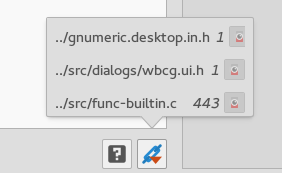
\includegraphics[width=0.4\textwidth]{img/gsoc2_it2_ui3.png} 
    \caption{}
    \label{fig:gsoc2_it2_ui2}
\end{figure}

Por último engadese na interface a opción de obter os orixes de cada mensaxe. Podemos ver esta modificación na Figura~\ref{fig:gsoc2_it2_ui1}.


\subsubsection{Bindings Gettext-PO}
Os bindings da biblioteca gettext-po non permitían gardar un ficheiro e seguir traballando con el. Tras analizar o código C xenerado polo compilador de Vala demonos conta de que se trataba dun problema de xestión de memoria. Ao gardar un ficheiro, liberabase a memoria empregada por este e, polo tanto, ó volver intentar editalo o programa cerrábase debido a un fallo de segmentación. Solucionamos isto modificando as opcións de xestión de memoria dos bindings e así permitimos gardar os cambios.

Ademais tamén implementamos a xestión de cabeceiras de ficheiros gettext-po desta forma cos métodos \emph{get\_info} e \emph{set\_info} podemos acceder a cabeceira desta mensaxe e actualizar a información de forma correcta no momento de gardar un ficheiro.

\subsubsection{Reportes e Feedback}

Escribese un\footnote{\href{http://aquelando.info/keep-working-on-gnomecat/}{Keep working on GNOMECAT}} reporte.

\subsubsection{Tarefas e seguimento}

As tarefas realizadas durante esta iteración foron:

\begin{itemize}
  \item Atallos de teclado.
  \item Interface de Usuario.
  \item Bindings Gettext-PO.
    \begin{itemize}
      \item Xestión de cabeceiras.
      \item Gardado de ficheiros.
    \end{itemize}
\end{itemize}


\subsection{Terceira Iteración: Perfiles de usuario e interface}
Esta iteración dura dende o 7 de Xullo ao 16 do mesmo mes. Melloramos algo a interface de usuario e implementamos algún detalle que faltaba no sistema de perfiles.

\subsubsection{Interface de usuario: Barra de notificación}
Necesitabamos un mecanismo par avisar ao usuario de certos eventos na interface como cando os parametros de busca empregador non xeneran ningún resultado, ou cando estamos navegando a través das mensaxes e chegamos a última. Para facer isto incorporamos un GtkInfoBar na interface e implementamos os métodos \emph{show\_notification} e \emph{hide\_notification} para amosar e esconder as notificacións. As notificacións amosanse durante un periodo de 3 segundos e despois ocultanse. Na Figura~\ref{fig:gsoc2_it3_ui} pódese ver o resultado.

\begin{figure}[h!]
    \centering
    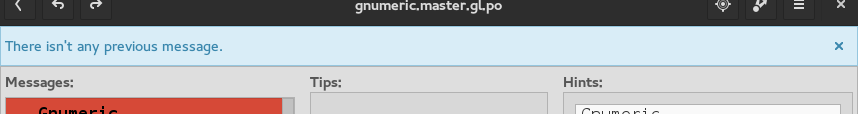
\includegraphics[width=0.8\textwidth]{img/gsoc2_it3_ui.png}
    \caption{Barra de notificacións}
    \label{fig:gsoc2_it3_ui}
\end{figure}

\subsubsection{Perfiles de usuario}
Ata este momento o perfil activo era o primeiro que se creara polo que tivemos que implementar a funcionalidade de activar un perfil. Ademais tamén imlementamos a posibilidade de borrar un perfil. Todas estas novas funcións tiveron o seu reflexo na interface na que apareceron novos botóns para borrar e activar perfiles.

\subsubsection{Reportes e Feedback}

Escribese un\footnote{\href{http://aquelando.info/details-and-more-details/}{Details and more details}}.

\subsubsection{Tarefas e seguimento}

As tarefas realizadas durante esta iteración foron:

\begin{itemize}
  \item Interface de usuario: barra de notificación.
  \item Perfiles de usuario.
    \begin {itemize}
      \item Función borrar perfil.
      \item Función activar perfil.
    \end{itemize}
  \item Modificar ficheiro das formas plurais.
\end{itemize}

\subsection{Cuarta Iteración: Plugins e GUADEC} %14 July - 27 July
Esta iteración dura dende o 16 de Xullo ata o 5 de Agosto tendo a GUADEC polo medio. Conseguimos implementar o motor de plugins e creamos algúns plugins de exemplo.

\subsubsection{Plugins}
Incorporamos un motor de plugins empregando a biblioteca LibPeas ademais modificamos so scripts de Autotools para que compile os plugins. Por outra parte refactorizamos moitas clases do núcleo do programa para que deixen de depender da interface gráfica e podelas incluir nunha pequena biblioteca para os plugins que imos crear.

\subsubsection{Presentación GUADEC 2014 (Strasbourg)}
Da mesma forma que na edición anterior acudimos a GUADEC, a reunión de programadores e usuarios de GNOME en Europa. Desta vez celebrase en Strasbourg.

\begin{figure}[h!]
    \centering
    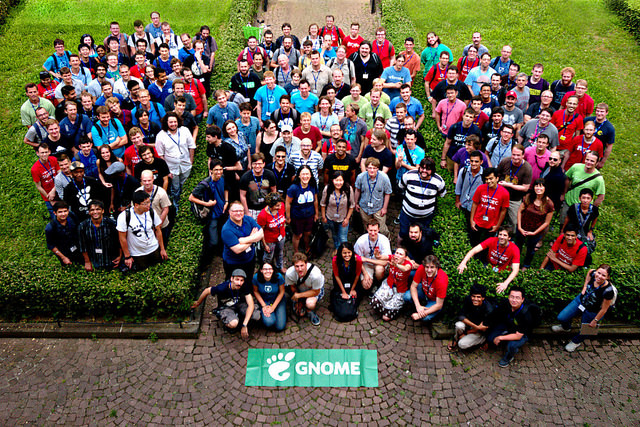
\includegraphics[width=0.999\textwidth]{img/guadec_2014.jpg}
    \caption{GUADEC 2014 (Strasbourg)}
    \label{fig:guadec2012}
\end{figure}

Tamén temos a oportunidade de presentar o proxecto ante a comunidade GNOME nunha charla lóstrego de 3 minutos onde explicaremos os novos cambios na interface, a implementación e plugins e as novas características implementadas.

\subsubsection{Reportes e Feedback}

Escribese un\footnote{\href{http://aquelando.info/api-guadec-and-big-files/}{API, GUADEC and big files}} reporte.

\subsubsection{Tarefas e seguimento}

As tarefas realizadas duarnte esta iteración foron:

\begin{itemize}
  \item Melloras en Autools
  \item Interface de usuario: \emph{scrolling} nas buscas.
  \item Implementación de plugins.
  \item Refactorizar clase File: evitar dependencias coa interface.
\end{itemize}

\subsection{Quinta Iteración: Detalles finais e escribir documentación}
Esta iteración dura dende o 5 de Agosto ata o 17 do mesmo mes. Nela puliremos algún detalle da interface e melloraremos a calidade do código e a documentación.

\subsubsection{Documentación e limpar código}
Realizamos unha revisión do código para mellorar a súa calidade e a súa limpeza. Para iso aseguramonos de que todos os ficheiros teñen a licencia declarada no cabezallo do mesmo, que estamos empregando espacios en vez de tabuladores e que todo o código segue un mesmo estilo.

Ademais actualizamos a documentación que tiñamos e creamos algunha nova. Creamos uns novos diagramas UML para os cambios feitos durante esta edición do Google Summer of Code e escribimos información explicando algún dos conceptos empregados no programa.

\subsubsection{Interface: Lista de mensaxes e estatisticas do documento.}
Dende a pasada edición do Google Summer of Code tiñamos detectado que o programa funcionaba moi lento cando intentabamos abrir un ficheiro con un número moi grande de cadeas. Tras varios intentos fallidos para solucionar este erro demonos conta de que o problema era que o widget GtkListBox non soportaba un número tan grande de filas. Substituímos dito widget por un TreeView e implementamos un GtkCellRenderer personalizado. Con isto obtemos un resulado moi semellante ao de anterior pero sendo esta implementación moito máis fluída.

\begin{figure}[h!]
    \centering
    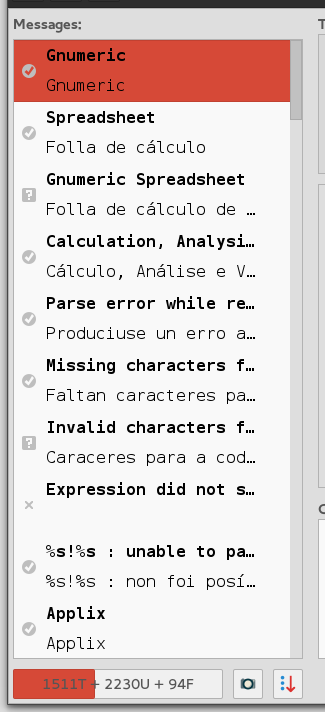
\includegraphics[width=0.3\textwidth]{img/gsoc2_it5_ui.png}
    \caption{Lista de Mensaxes e estatisticas}
    \label{fig:gsoc2_it5_ui}
\end{figure}

Ademais implementamos a opción de filtrar as mensaxes para que o usuario poida dicir que solo quere ver as mensaxes que están traducidas ou as mensaxes que están sen traducir e, tamén, a posibilidade de ordenar as mensaxes por estado. Na Figura~\ref{fig:gsoc2_it5_ui} podemos ver a nova lista de mensaxes coas funcións anteriores implementadas.

Ademais incluimos na interface unha barra de progreso onde se indica a cantidade de cadeas traducidas, sen traducir e con tradución difusa.

\subsubsection{Reportes e Feedback}
Nesta ocasión non se escriben reportes mais si que recibimos feedback de algún traductor a través do correo electronico. As cousas queestes traductores consideran que se deben mellorar son as seguintes:

\begin{itemize}
  \item Mellora dos atallos de teclado.
\end{itemize}

\subsubsection{Tarefas e seguimento}

As tarefas realizadas durante esta iteración foron:

\begin{itemize}
  \item Documentación.
  \item Limpar código.
  \item Interface de usuario: Refactorizar lista de mensaxes.
    \begin{itemize}
      \item Implementar filtros para lista de mensaxes.
      \item Implementar a función de ordenar para mensaxes.
    \end{itemize}
  \item Melloras en Autotools.
\end{itemize}

\subsection{Estado ao fin do GSoC 2014}

\section{Segundo cuatrimestre 2014/2015}
